\subsection{Sorgente}

La sorgente \am{} emette $\alpha$ a due energie cinetiche\footnote{PDG 2016 \S{} 37.}: \SI{5.443}{MeV}, \SI{5.486}{MeV}.
La sorgente emette anche raggi $\gamma$ a \SI{60}{keV} (\SI{36}\%),
per i quali la lunghezza di attenuazione nel silicio è circa\footnote{PDG 2016 fig. 33.18.}
$\SI{3}{g\,cm^{-2}} / \SI{2.6}{g\,cm^{-3}} = \SI{1.1}{cm}$.
Lo spessore del rivelatore è dell'ordine dei \si{\micro m}
e i fotoni vengono assorbiti con una probabilità circa del \SI{50}\%\footnote{NIST XCOM \url{https://physics.nist.gov/PhysRefData/Xcom/html/xcom1.html}.},
allora la probabilità di assorbimento è circa \SI{1/20000}{\micro m^{-1}}.
Dalla scheda sappiamo l'area del fotodiodo (\SI{20}{mm^2})
e la distanza della sorgente dal fotodiodo ad angolo \SI0{\degree} è \SI{6}{cm},
quindi il rate atteso di fotoni che rilasciano tutta l'energia è
$\SI{315}{kBq} \times \SI{36}\% \times \SI{20}{mm^2} / (4 \pi (\SI{6}{cm})^2) \times \SI{1/20000}{\micro m^{-1}}
= \SI{0.003}{s^{-1}\,\micro m^{-1}}$.
Bisogna poi vedere se l'energia dei fotoni è sufficiente a superare la soglia del discriminatore.

\subsection{Scattering Rutherford}

La sezione d'urto differenziale in approssimazione non relativistica di una particella di carica $+ze$ ed energia cinetica $T$ su un campo elettrostatico di carica $+Ze$ è\footnote{Wikipedia: Rutherford scattering \url{https://en.wikipedia.org/wiki/Rutherford_scattering}.}
%\marginpar{non mi sembra il caso di citare qualcosa per questa formula, men che meno wikipedia (Bob)} % sti...
\begin{equation}
	\label{eq:rutherford}
	\dv\sigma\Omega = \left( \frac {zZ\alpha\hbar c} {2T(1-\cos\theta)} \right)^2.
\end{equation}
Per un campo generato da una massa $M$ di carica $+Ze$,
applicando nella \eqref{eq:rutherford} le trasformazioni del problema in coordinate relative con la massa ridotta
(vedi \autoref{sec:conti}),
con $m$ massa della particella incidente e $T_\text{in}$, $T_\text{out}$ energia cinetica rispettivamente prima e dopo l'interazione, si ottiene
\begin{align}
	T_\text{out}
	&= T_\text{in} \left( 1 - 2\frac mM(1-\cos\theta) + O\left(\frac mM\right)^2 \right),
	\label{eq:tout} \\
	\dv\sigma\Omega &= \left( \frac {zZ\alpha\hbar c} {2T_\text{in}(1-\cos\theta)} \right)^2
	\left( 1 + O\left(\frac mM\right)^2 \right). \notag
\end{align}
Notiamo che la correzione al primo ordine nel rapporto delle masse alla sezione d'urto è nulla.

\subsection{Multiplo scattering}

Le particelle $\alpha$, passando nel bersaglio,
vengono in maggior parte deviate di piccoli angoli per interazione con molti atomi
e occasionalmente di un grande angolo per interazione con un singolo nucleo secondo la \eqref{eq:rutherford}.
Nel secondo caso comunque subiscono anche una deviazione ulteriore di un piccolo angolo
prima e dopo l'interazione ravvicinata con il nucleo.
La deviazione standard della distribuzione dei piccoli angoli,
nel limite non relativistico,
con l'angolo riferito a un piano fissato nello spazio anziché rispetto a un asse,
è data da\footnote{PDG 2016 \S{} 33.3.}
\begin{equation}
	\label{eq:ms}
	\theta_0 = \frac {\SI{6.8}{MeV}} {T_\text{in}} z \sqrt{\frac{x}{X_0}} \left(1+0.038\log\frac x{X_0}\right)
\end{equation}
dove $x$ è lo spessore attraversato e $X_0$ è la lunghezza di radiazione,
che vale\footnote{PDG 2016 \S{} 6.} \SI{8.9}{cm} per l'alluminio e \SI{0.33}{cm} per l'oro.
Ad esempio con $x = \SI5{\micro m}$ e $T_\text{in} = \SI5{MeV}$
risulta $\theta_0 = \SI{9}\degree$ per l'oro e \SI{1.5}{\degree} per l'alluminio.

\subsection{Simulazione}

\begin{figure}
	\centering
	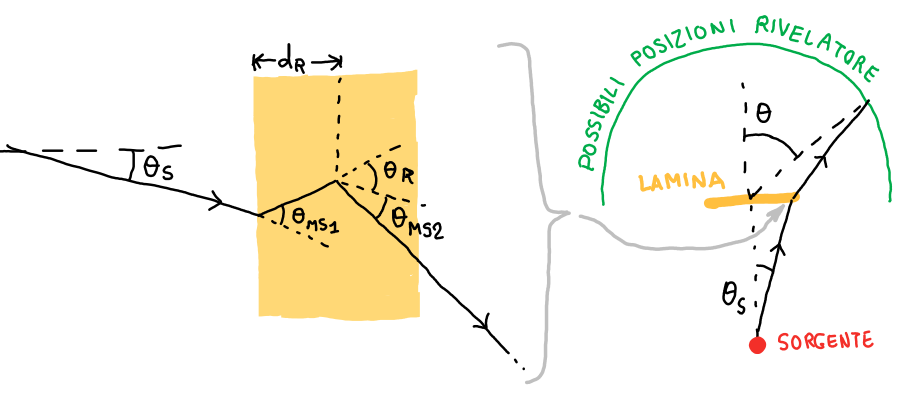
\includegraphics[width=\textwidth]{immagini/schemamc}
	\caption{\label{fig:schemamc}
	Schema della simulazione.
	Il raggio esce dalla sorgente con un angolo $\theta_S$,
	fa multiplo scattering di $\theta_\text{MS1}$,
	scattering Rutherford $\theta_R$ alla profondità $d_R$
	e di nuovo multiplo scattering $\theta_\text{MS2}$.
	L'angolo a cui bisognerebbe mettere il rivelatore per osservare la traiettoria simulata è $\theta$,
	che dipende solo da $\theta_S$.}
\end{figure}

Implementiamo una simulazione 2D semplificata dell'esperimento,
illustrata in \autoref{fig:schemamc}.
Passaggi della simulazione:
\begin{enumerate}
	\item
	Partiamo con un'energia di \SI{5.46}{MeV}
	e simuliamo la perdita di energia nei \SI{3}{\micro m} di oro che incapsulano la sorgente.
	La perdita di energia è calcolata da $\mathrm dE/\mathrm dx$ tabulati\footnotemark,
	\footnotetext{NIST ASTAR \url{https://physics.nist.gov/PhysRefData/Star/Text/ASTAR.html}.}
	integrati per passi discreti di \SI{0.5}{\micro m};
	alla perdita di energia è aggiunta una variazione casuale gaussiana di deviazione standard \SI{10}\%.
	\item
	Estraiamo un angolo di uscita dalla sorgente $\theta_S$ con distribuzione uniforme
	delimitata dalla larghezza del collimatore.
	L'uniformità è giustificata dalla larghezza del fascio (vedi \autoref{sec:forma}). 
	\item
	Estraiamo uniformemente la profondità nel bersaglio $d_R$ a cui faremo avvenire lo scattering Rutherford.
	\item
	Simuliamo la perdita di energia fino alla profondità $d_R$
	e deviamo la traiettoria di un angolo di multiplo scattering $\theta_\text{MS1}$
	estratto da una gaussiana di deviazione standard $\theta_0$ (\autoref{eq:ms}).
	\item
	Estraiamo il coseno dell'angolo di scattering Rutherford $\theta_R$
	dalla distribuzione $(1-\cos\theta_R)^{-1}$,
	tagliata a $\theta_R>\epsilon$ dove $\epsilon$ è un parametro della simulazione.
	Calcoliamo l'energia persa con la \eqref{eq:tout}.
	Salviamo il peso statistico $w = (T_\text{in}^2 (1-\cos\theta_R))^{-1}$
	per tenere conto della distribuzione delle energie a cui avviene lo scattering
	e della distribuzione con cui abbiamo estratto $\theta_R$.
	\item
	Simuliamo perdita di energia e multiplo scattering fino all'uscita dal bersaglio.
	\item
	Troviamo l'intersezione della traiettoria finale con la circonferenza delle possibili posizioni del rivelatore,
	da cui calcoliamo l'angolo $\theta$ che è quello che impostiamo nell'esperimento.
	\item
	Moltiplichiamo i pesi $w$ per un fattore globale
	$Z^2 \cdot \max \theta_S \cdot d / N$,
	dove $d$ è lo spessore del bersaglio
	e $N$ è il numero di particelle simulate,
	che in generale è maggiore del numero di campioni finali
	perché le particelle si possono fermare per perdita di energia.
	\item
	Facciamo un istogramma degli eventi simulati nella variabile $\theta$,
	contando ogni evento non come +1 ma con il suo peso $w$.
\end{enumerate}
I pesi $w$ forniscono la corretta normalizzazione per il rate a grande angolo.
Il rate a piccolo angolo è in pratica impostato dal parametro regolarizzatore $\epsilon$.

\begin{figure}
	\centering
	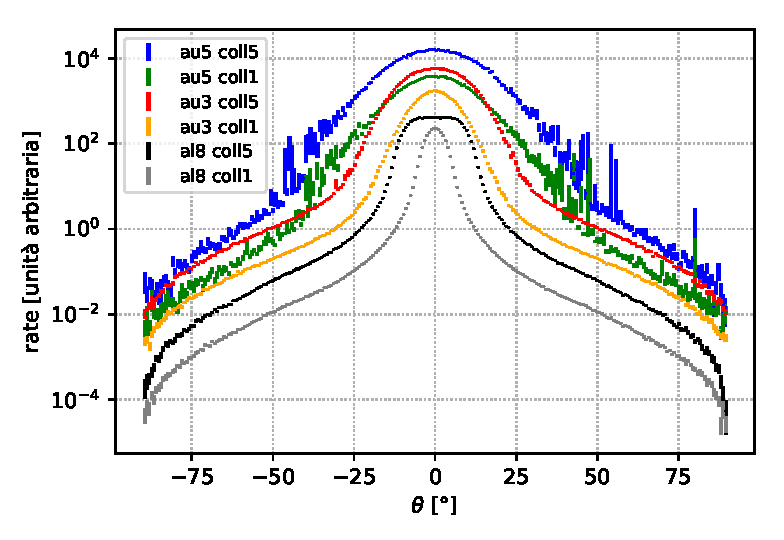
\includegraphics[width=30em]{immagini/mc}
	\caption{\label{fig:mc}
	Simulazione per le varie configurazioni elemento-spessore-collimatore.
	Per ogni configurazione sono state simulate \num{1000000} particelle rivelate,
	con $\epsilon=\SI{1}{\degree}$,
	e istogrammate in 250 bin in $\theta$.}
\end{figure}
